\section{Architecture}
\label{sec:architecture}

This chapter describes the architecture of Stress+.
The whole architecture was designed in a way that arbitrary stress tests with different modules can be created very easily.
It was also taken into account that programming and adding new modules is very simple.
Each stress test consists of a pipeline of screens which are shown to the patient successively in the specified order.
Additionally, a stress test can contain overlays which are displayed on top of the screens.

\begin{figure}[htb]
  \centering
  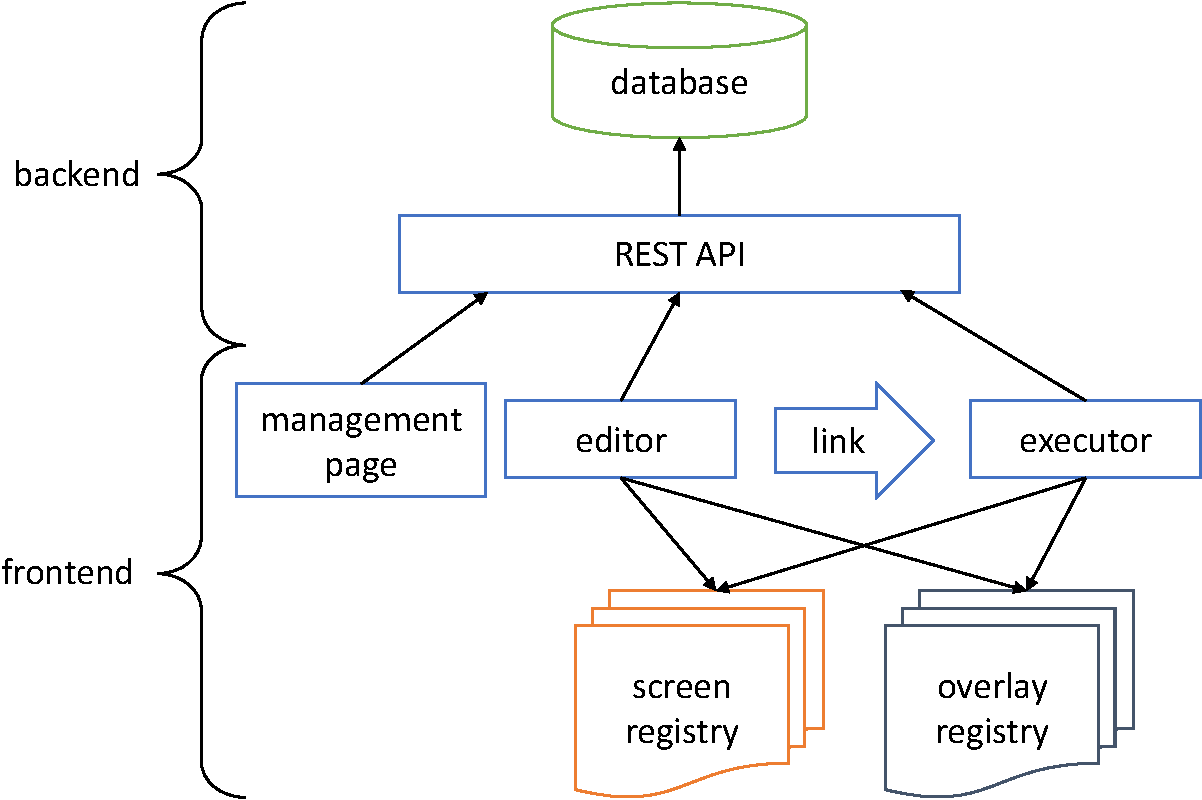
\includegraphics[width=\textwidth]{figures/Architecture-crop}
  \caption{Software architecture}
  \label{fig:software-architecture}
\end{figure}

The figure \ref{fig:software-architecture} shows the software architecture of Stress+, which developed as a browser-based application and consists of a frontend and a backend.
The main frontend components of Stress+ are the \textit{Editor} for creating and editing stress tests and the \textit{Executor} for executing a stress test.
On the \textit{Management page} all available stress tests can be managed.
To be able to easily add new modules in the future all available screens and overlays are registered in the \textit{Screen registry} and \textit{Overlay registry}. 
Therefore the \textit{Editor} and \textit{Executor} are developed generically and must query the registries to know which modules are currently present.
After saving a stress test in the \textit{Editor} a link is generated, which can be sent to the patient so he can execute the stress test.

The backend is responsible for saving the stress test configurations and the statistics on how the patient performed.
Therefore it consists of a REST API, through which the database can be accessed.

\subsection{Frontend}
The frontend is a single-page application written in JavaScript utilizing the React framework. 
The following sections describe the different frontend components in more detail.

\subsubsection*{Screen}
The stress test consists of a list of screens that will be displayed successively to the patient. 
A screen will be displayed fullscreen inside the user's browser. 
Each screen has its own settings, which can be adjusted inside the editor. 
All available screens can be found in chapter \ref{sec:screens}.

\subsubsection*{Overlay}
The stress test can be equipped with overlays that are displayed on top of the current screen. 
All overlays are displayed simultaneously during the whole stress pipeline execution, therefore they do not have an order. 
Each overlay has its own settings, which can be adjusted inside the editor.
All available overlays can be found in chapter \ref{sec:overlays}.

\subsubsection*{Management page}
On the management page, all available stress test are displayed.
From there you can open a stress test in the editor, delete one or create a new test.
Further details about the management page can be found in chapter \ref{sec:management-page}.

\subsubsection*{Editor}
The stress tests can be created and edited in the editor.
Also, every setting of the screens and overlays can be adjusted within the editor.
Each stress test has a unique id that is generated when it is saved for the first time.
With this id a link is generated that can be sent to patients so they can execute the stress test.
From the editor, users can also download all recorded statistics for the current stress test.
Further details about the editor can be found in chapter \ref{sec:editor}.

\subsubsection*{Executor}
The executor is responsible for executing the stress test specified by the link.
It will display each screen successively to the patient and show all overlays simultaneously during the whole stress test run.
The executor also collects records from the screens and persist them in the database.
Further details can be found in chapter \ref{sec:executor}.

\subsection{Backend}
The backend consists of the Database and the REST API

\subsubsection*{Database}
To save the stress test configurations and the results of a stress test executions a database is used.
The data does not have a clear structure, as arbitrary modules can be composed together in a stress test.
Therefore, the document-oriented NoSQL database MongoDB is used instead of a relational database.

\subsubsection*{REST API}
The REST API acts as the connection between the frontend and the database.
It can be accessed via HTTP and uses JSON documents for transferring the data.
The REST API endpoints are written in JavaScript on the NodeJS platform.
